% -----------------------------------------------
% Template for ISMIR Papers
% 2017 version, based on previous ISMIR templates

% Requirements :
% * 6+n page length maximum
% * 4MB maximum file size
% * Copyright note must appear in the bottom left corner of first page
% * Clearer statement about citing own work in anonymized submission
% (see conference website for additional details)
% -----------------------------------------------

% Anonymity: authors, GitHub links, acknowledgments

\documentclass{article}
\usepackage[T1]{fontenc} \usepackage[utf8]{inputenc}
\usepackage[svgnames]{xcolor}
\usepackage[bookmarks=false,colorlinks=true,allcolors=DarkBlue]{hyperref} % MidnightBlue, NavyBlue, DarkBlue, Maroon
\usepackage{ismir,amsmath}
\usepackage{graphicx} \graphicspath{{figs/}}
\usepackage{booktabs, threeparttable, tabularx}
\usepackage{enumitem} \setlist{itemsep=0pt,topsep=0pt,parsep=0pt,partopsep=0pt}

\newcommand{\todo}[1]{{\color{red} #1}}

\newcommand{\ntracks}{106,574 }
\newcommand{\nartists}{16,341 }
\newcommand{\nalbums}{14,854 }
\newcommand{\ngenres}{161 }
\newcommand{\tduration}{343 }
\newcommand{\aduration}{278 }
\newcommand{\size}{900 }

\newcommand{\tspacea}{\hspace{0.7em}}
\newcommand{\tspaceb}{\hspace{0.9em}}

\title{FMA: A Dataset For Music Analysis}

\multauthor
{Michaël Defferrard \hspace{.6cm} Kirell Benzi \hspace{.6cm} Pierre Vandergheynst \hspace{.6cm} Xavier Bresson$^1$}
{
	LTS2, EPFL, Lausanne, Switzerland \hspace{1cm}
	{\small$^1$XB is now at NTU, Singapore. Work conducted when he was at EPFL.}\\
	{\tt\small \{michael.defferrard,kirell.benzi,pierre.vandergheynst\}@epfl.ch, xbresson@ntu.edu.sg}
  }

%\multauthor
%{$^1$ \hspace{1cm} Second author$^1$ \hspace{1cm} Third author$^2$} { \bfseries{Fourth author$^3$ \hspace{1cm} Fifth author$^2$ \hspace{1cm} Sixth author$^1$}\\
%  $^1$ Department of Computer Science, University , Country\\
%$^2$ International Laboratories, City, Country\\
%$^3$  Company, Address\\
%{\tt\small CorrespondenceAuthor@ismir.edu, PossibleOtherAuthor@ismir.edu}
%}
%\def\authorname{First author, Second author, Third author, Fourth author, Fifth author, Sixth author}

%\threeauthors
%  {First Author} {Affiliation1 \\ {\tt author1@ismir.edu}}
%  {Second Author} {\bf Retain these fake authors in\\\bf submission to preserve the formatting}
%  {Third Author} {Affiliation3 \\ {\tt author3@ismir.edu}}

%% To make customize author list in Creative Common license, uncomment and customize the next line
\def\authorname{Kirell Benzi, Michaël Defferrard, Pierre Vandergheynst, Xavier Bresson}

\sloppy % please retain sloppy command for improved formatting
\begin{document}
\maketitle

% about 150-200 words.
\begin{abstract}
The Free Music Archive (FMA) is an open and easily accessible dataset that can be used to evaluate several tasks in music information retrieval (MIR).
% TODO: which tasks
While content-based MIR tasks have typically been solved with feature engineering,
%with a two-stage approach: engineered features are extracted from music audio signals, and are then used as input to a regressor or classifier.
the community is becoming interested in feature learning and end-to-end learning. %, i.e. learning from signals to labels
That endeavor is however restrained by the limited availability of large audio datasets.
% The primary goal of this dataset is to enable the training of large models, which require lots of training data, which could potentially avert the semantic gap currently observed between the extracted low-level features such as MFCCs and the high-level targets such as genre.
By releasing the FMA we hope to foster research which will improve the state-of-the-art in several tasks and hopefully surpass the performance ceiling observed in e.g. genre recognition (MGR).
% as it happened in computer vision with the release of ImageNet.
The released data is composed of \ntracks tracks, \nartists artists, \nalbums albums, \ngenres genres, for a total of \tduration days of audio and \size GiB, all under permissive Creative Commons licenses.
It features a collection of metadata such as the song title, album, artist name and genres; user data such as play counts and favorites; free-form text such as description, biography and tags; together with full-length and high-quality audio as well as some pre-computed features. We propose a train/validation/test split and three subsets: a small genre-balanced dataset of 8,000 songs from 8 major genres, a medium genre-unbalanced dataset of 25,000 songs from 16 genres, and a 90 GiB version of the full set with clips trimmed to 30s.
This paper describes the dataset and how it was created, proposes some tasks, and evaluates some baselines for MGR.
% Xavier: tasks, such as ...
Code, data, and usage examples are available at \url{https://github.com/mdeff/fma}.
%All the code to create,  as well as links to download the data and usage examples are available at \url{https://github.com/mdeff/fma}.

% Our major goal is to go beyond the existing limitations of available music datasets, which are either the small size of datasets with raw audio tracks, the availability and legality of the music data, or the lack of metadata for artists analysis or song ratings for recommender systems. Existing datasets such as GTZAN, TagATune, and Million Song suffer from the previous limitations. It is however essential to establish such benchmark datasets to advance the field of music analysis, like the ImageNet dataset which made possible the large success of deep learning techniques in computer vision.

% which contains 77,643 songs and 68 genres spanning 26.9 days of song listening
\end{abstract}


%%%%%%%%%%%%%%%%%%%%%%%%%%%%%%%%%%%%%%%%%%%%%%%%%%%%%%%%%%%%%%%%%%%%%%%%%%%%%%%%
\section{Introduction} % and Motivation}
%%%%%%%%%%%%%%%%%%%%%%%%%%%%%%%%%%%%%%%%%%%%%%%%%%%%%%%%%%%%%%%%%%%%%%%%%%%%%%%%


% hook
While the development of new mathematical models and algorithms to solve challenging real-world problems is obviously of first importance to any field of research, evaluation and comparison to the existing state-of-the-art is necessary for a technique to be widely adopted by research communities. Such tasks require open benchmark datasets to be reproducible. % to achieve their purpose, which are sometimes challenging to collect and share.
In computer vision, the community has developed over the years established benchmark datasets such as \href{http://yann.lecun.com/exdb/mnist/}{MNIST} \cite{mnist}, \href{https://www.cs.toronto.edu/~kriz/cifar.html}{CIFAR} \cite{cifar}, or \href{http://www.image-net.org}{ImageNet} \cite{imagenet}. These datasets are free, legal, easily available, and have proved essential to advance the field. The most celebrated example, the \href{http://www.image-net.org/challenges/LSVRC/2012/}{ILSVRC2012 challenge} on an unprecedented ImageNet subset of 1.3M images \cite{imagenet_challenge}, demonstrated the power of deep learning (DL), which won the competition with an 11\% accuracy advantage over the second best \cite{convnet_imagenet}, and unlocked incredible achievements in both fields \cite{dl}.

\begin{table}[t]
	\centering
	\begin{threeparttable}
	\begin{tabular}{l@{ }rrcc}
		\toprule
		dataset\tnote{1} & \#clips & \#artists & year & audio \\
		\midrule
		\href{https://staff.aist.go.jp/m.goto/RWC-MDB/}{RWC} \cite{RWC} & 465 & - & 2001 & yes \\
		\href{http://calab1.ucsd.edu/~datasets/cal500/}{CAL500} \cite{cal500} & 500 & 500 & 2007 & yes \\
		\href{http://mtg.upf.edu/ismir2004/contest/tempoContest/node5.html}{Ballroom} \cite{ballroom} & 698 & - & 2004 & yes \\
		\href{http://ismir2004.ismir.net/genre_contest/}{ISMIR2004} & 729 & - & 2004 & yes \\
		\href{https://marsyasweb.appspot.com/download/data_sets/}{GZTAN} \cite{gtzan} & 1,000 & $\sim300$ & 2002 & yes \\
		\href{http://www.cp.jku.at/datasets/musiclef/}{MusiClef} \cite{musiclef} & 1,355 & 218 & 2012 & yes \\
		\href{https://labrosa.ee.columbia.edu/projects/artistid/}{Artist20} \cite{artist20} & 1,413 & 20 & 2007 & yes \\
		\href{http://www-ai.cs.uni-dortmund.de/audio.html}{Homburg} \cite{homburg} & 1,886 & 1,463 & 2005 & yes \\  % GarageBand
		103-Artists \cite{103artists} & 2,445 & 103 & 2005 & yes \\
		\href{http://www.seyerlehner.info/index.php?p=1_3_Download}{Unique} \cite{unique} & 3,115 & 3,115 & 2010 & yes \\
		\href{http://www.seyerlehner.info/index.php?p=1_3_Download}{1517-Artists} \cite{1517artists} & 3,180 & 1,517 & 2008 & yes \\
		\href{http://www.ppgia.pucpr.br/~silla/lmd/}{LMD} \cite{lmd} & 3,227 & - & 2007 & no \\
		\href{http://anasynth.ircam.fr/home/media/ExtendedBallroom}{EBallroom} \cite{extballroom} & 4,180 & - & 2016 & no\tnote{2} \\
		\href{https://labrosa.ee.columbia.edu/projects/musicsim/uspop2002.html}{USPOP} \cite{uspop} & 8,752 & 400 & 2003 & no \\
		\href{http://calab1.ucsd.edu/~datasets/cal10k/}{CAL10k} \cite{cal10k} & 10,271 & 4,597 & 2010 & no \\ % Swat10k
		\href{http://mirg.city.ac.uk/codeapps/the-magnatagatune-dataset}{TagATune} \cite{magnatagatune} & 25,863\tnote{3} & 230 & 2009 & yes\tnote{4} \\ % MagnaTagATune
		\href{http://jmir.sourceforge.net/index_Codaich.html}{Codaich} \cite{codaich} & 26,420 & 1,941 & 2006 & no \\ % paper 20,849
		\bf \href{https://github.com/mdeff/fma/}{FMA} & \bf \ntracks & \bf \nartists & \bf 2017 & \bf yes \\
		\href{http://www.omras2.org/}{OMRAS2} \cite{omras} & 152,410 & 6,938 & 2009 & no \\
		\href{https://labrosa.ee.columbia.edu/millionsong/}{MSD} \cite{msd} & 1,000,000 & 44,745 & 2011 & no\tnote{2} \\
		\href{https://research.google.com/audioset/}{AudioSet} \cite{audioset} & 2,084,320 & - & 2017 & no\tnote{2} \\
		\bottomrule
	\end{tabular}
	\begin{tablenotes}
		% 103-Artists is also known as DB-L, Extended Ballroom
		\item[1] Names are links to datasets' homepage.
		\item[2] Audio can be downloaded from \href{http://www.ballroomdancers.com}{ballroomdancers.com}, \href{https://www.7digital.com}{7digital.com}, \href{https://www.youtube.com}{youtube.com}.
		\item[3] The 25,863 clips are cut from 5,405 songs.
		\item[4] Low quality 16 kHz, 32kbps, mono mp3.
	\end{tablenotes}
	\end{threeparttable}
	\caption{Comparison with some other datasets.} % Genre classification datasets.
	\label{tab:datasets}
\end{table}
% Lists of datasets:
% * http://www.audiocontentanalysis.org/data-sets/
% * A Survey of Evaluation in Music Genre Recognition

\begin{table*}[t]
	\centering
	\begin{threeparttable}
		\begin{tabular}{l@{\hspace{2.7em}}r
			@{\hspace{2.7em}}>{$}r<{$}
			@{}>{${}={}$}c@{}
			>{$}l<{$}
			@{\hspace{2.7em}}>{$}c<{$}
			@{\hspace{2.7em}}c@{\hspace{2.7em}}c}
		\toprule
		dataset & \#samples & \multicolumn{3}{c}{dimensionality} & \multicolumn{3}{c}{size} \\
		\cmidrule{6-8}
				&           & \multicolumn{3}{c}{}               & \text{scale} & [GB] & [days] \\
		\midrule
		\href{http://mirg.city.ac.uk/codeapps/the-magnatagatune-dataset}{TagATune} \cite{magnatagatune} &
			25,863 & 29\cdot16\cdot10^3\cdot1 && 4.6\cdot10^5 & 1.2\cdot10^{10} & 3 & 8.7 \\ % MagnaTagATune
		\href{https://research.google.com/audioset/}{AudioSet} \cite{audioset} \tnote{1} &
			2,084,320 & 10\cdot44\cdot10^3\cdot2 && 8.8\cdot10^5 & 1.8\cdot10^{12} & - & 241 \\
		\href{https://labrosa.ee.columbia.edu/millionsong/}{MSD} \cite{msd} \tnote{2} &
			1,000,000 & 49\cdot27\cdot10^3\cdot2 && 2.6\cdot10^6 & 2.6\cdot10^{12} & 625 & 541 \\
		\href{https://github.com/mdeff/fma/}{FMA} \tnote{2} &
			\ntracks & \aduration\cdot44\cdot10^3\cdot2 && 2.4\cdot10^7 & 2.6\cdot10^{12} & \size & \tduration \\
		\midrule
		\href{http://yann.lecun.com/exdb/mnist/}{MNIST} \cite{mnist} &
			70,000 & 28\cdot28\cdot1 && 7.8\cdot10^2 & 5.5\cdot10^{7\phantom0} & 0.011 & - \\
		\href{https://www.cs.toronto.edu/~kriz/cifar.html}{CIFAR-10} \cite{cifar} &
			60,000 & 32\cdot32\cdot3 && 3.0\cdot10^3 & 1.8\cdot10^{8\phantom0} & 0.16 & - \\
		\href{http://www.image-net.org/challenges/LSVRC/2012/}{ILSVRC 2012-17} \cite{imagenet_challenge} \tnote{3,4} &
			1,341,167 & 482\cdot415\cdot3 && 6.0\cdot10^5 & 8.0\cdot10^{11} & 100 & - \\
		\href{http://www.image-net.org}{ImageNet} \cite{imagenet} \tnote{3} &
			14,197,122 & 482\cdot415\cdot3 && 6.0\cdot10^5 & 8.5\cdot10^{12} & 1000 & - \\
		\bottomrule
	\end{tabular}
	\begin{tablenotes}
		\item[1] \href{https://support.google.com/youtube/answer/6039860}{YouTube recommended} sample rate for music videos.
		\item[2] Average duration and sample rate. Most excerpts from \href{https://www.7digital.com}{7digital} are 30 or 60s and 22 or 44kHz \cite{msd_features}.
		\item[3] Average resolutions. Most applications resize or crop to $256\cdot256$ for a scale of $2.6\cdot10^{11}$ and $2.8\cdot10^{12}$.
		\item[4] Object detection / classification task. It is the most used dataset for image classification.
	\end{tablenotes}
	\end{threeparttable}
	\caption{Comparison between the largest public audio and image datasets. Dimensionality is (length $\cdot$ sample rate $\cdot$ \#channels) for audio and (xdim $\cdot$ ydim $\cdot$ \#channels) for images. Scale is the number of samples times the dimensionality. Size is for a (zipped) archive of all \texttt{.mp3} or \texttt{.jpg} in GB, an indication of the quantity of information affected by the size and diversity of the data. The last column is the number of days necessary to listen to the whole available audio.}
	\label{tab:size}
\end{table*}
% Magnatagature dead links: http://tagatune.org/Datasets.html http://tagatune.org/Magnatagatune.html
% Announcement: https://musicmachinery.com/2009/04/01/magnatagatune-a-new-research-data-set-for-mir/

% Xavier: De meme pour Table 2, c'est interessant bien sur, mais encore une fois, les datasets de MSD et autres n'ont pas disponible (directement et facilement) les raw audio data. Cela rend confusing le main message. Aussi, je ne parlerais pas des MNIST, CIFAR et autres image datasets, ce n'est pas le point de ce papier, targeted music, et cela peut rendre notre message confusing.

\begin{figure*}
	\begin{minipage}{0.74\linewidth}
		\centering
		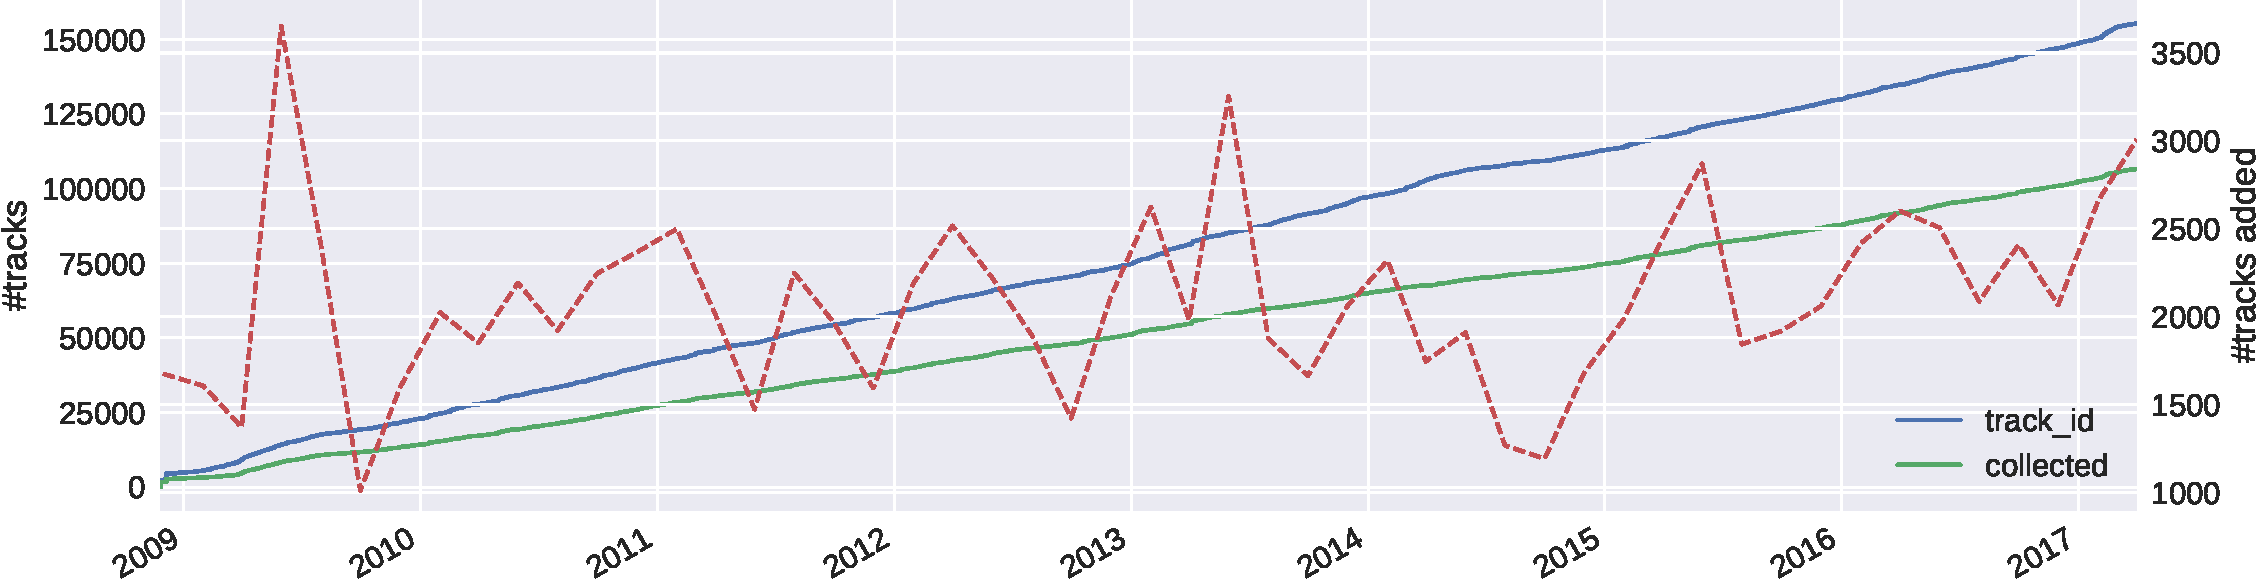
\includegraphics[width=\linewidth]{growth.pdf}
	\end{minipage} \hfill
	\begin{minipage}{0.24\linewidth}
		\centering
		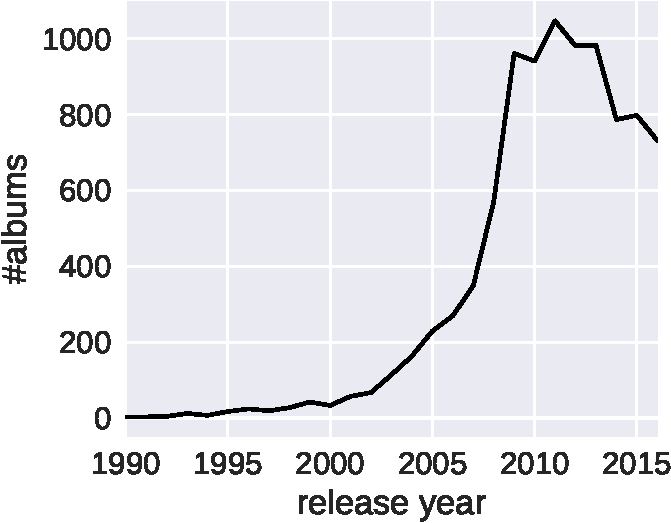
\includegraphics[width=\linewidth]{album_release_year.pdf}
	\end{minipage}
	\caption{(left) Growth of the archive, created in 11/2008. (right) Number of albums released per year, from 1902 to 2017.}
	\label{fig:growth}
	\label{fig:album_release_year}
\end{figure*}

\begin{table*}
	\tiny
	\centering
\begin{tabular}{@{}l@{\tspacea}l@{\tspacea}l@{\tspacea}l@{\tspacea}r@{\tspacea}r@{\tspacea}l@{\tspacea}r@{\tspacea}l@{\tspacea}l@{\tspacea}l@{}}
	\toprule
	\multicolumn{6}{@{}l}{track} & \multicolumn{3}{@{}l}{album} & \multicolumn{2}{@{}l}{artist} \\
	track\_id & title & genres\_all & genre\_top & dur. & listens & title & listens & tags & name & location \\
	\midrule
	150073 & Welcome to Asia & [2, 79] & International & 81 & 683 & Reprise & 4091 & [world music, dubtronica, fusion] & DubRaJah & Russia \\
	140943 & Sleepless Nights & [322, 5] & Classical & 246 & 1777 & Creative Commons Vol. 7 & 28900 & [classical, alternate, soundtrack, piano, ... & Dexter Britain & United Kingdom \\
	64604 & i dont want to die alone & [32, 38, 456] & Experimental & 138 & 830 & Summer Gut String & 7408 & [improvised, minimalist, noise, ... & Buildings and Mountains & Oneonta, NY \\
	23500 & A Life In A Day & [236, 286, 15] & Electronic & 264 & 1149 & A Life in a Day & 6691 & [idm, candlestick, romanian, candle, ... & Candlestickmaker & Romania \\
	131150 & Yeti-Bo-Betty & [25, 12, 85] & Rock & 124 & 183 & No Life After Crypts & 3594 & [richmond, fredericksburg, trash rock, ... & The Crypts! & Fredericksburg \\
	\bottomrule
	\end{tabular}
	\caption{Some rows and columns of the metadata table, stored in \texttt{tracks.csv}.}
	\label{tab:tracks}
\end{table*}

\begin{table}
	\centering
	\begin{tabular}{|llll|}
		\hline
		track\_id & title & number & \\
		information & language\_code & license & \\
		composer & publisher & lyricist & \\
		genres & genres\_all & genre\_top & \\
		duration & bit\_rate & interest & \\ %samplerate \\
		\#listens & \#comments & \#favorites & tags \\
		date\_created & date\_recorded & & \\
		\hline
		album\_id & title & type & \#tracks \\
		information & engineer & producer & \\
		\#listens & \#comments & \#favorites & tags \\
		date\_created & date\_released & & \\
		\hline
		artist\_id & name & & \\
		bio & members & \multicolumn{2}{l|}{associated\_labels} \\
		website & wikipedia\_page & \multicolumn{2}{l|}{related\_projects} \\
		location & longitude & latitude & \\
		& \#comments & \#favorites & tags \\
		date\_created & active\_year\_end & \multicolumn{2}{l|}{active\_year\_begin} \\
		\hline
	\end{tabular}
	\caption{List of available per-track, per-album and per-artist metadata, i.e. the columns of \texttt{tracks.csv}.}
	%Not all of them are filled for each track.\footnote{See }
	%\texttt{albums.csv} and \texttt{artists.csv}.}
	% genres.csv ?
	\label{tab:metadata}
\end{table}

% Besides, the most influential competition in the field of music analysis organized every year is the Music Information Retrieval Evaluation eXchange (MIREX).\href{http://www.music-ir.org/mirex/wiki/}{MIREX} proposes several important music analysis challenges such as song identification, tag classification, music similarity and retrieval, etc. However, participants do not have access to neither the test set, nor the important train set. They must upload their code to a website that will be evaluated by the organizers. In other words, participants cannot train their analysis models on any part of the dataset.

% {\bf Available music datasets and their limitations.}
Unlike other modalities such as images or text for which a wealth of content is available, the lack of a large-scale, complete and easily available dataset for MIR has hindered research on data-heavy models such as DL.
\tabref{tab:datasets} lists the most common datasets used for content-based MIR.
GTZAN \cite{gtzan}, a collection of 1000 songs from 10 genres, was the first publicly available benchmark MGR dataset. As a result, despites its flaws \cite{gtzan_critic_1}, it continues to be the most used dataset for MGR \cite{mgr_eval}. The main limitations of GTZAN is its illegality, small size, and missing metadata (no user ratings or even artist name and song title). % Each song is represented by a 22,050Hz Mono 16-bit wav audio file of 30sec.
Looking at \tabref{tab:datasets}, the well-known MagnaTagATune and the Million Song Dataset (MSD) as well as the newer AudioSet appear as contenders for a large-scale reference dataset. % They however each have limitations.
MagnaTagATune, which was collected from the \href{https://magnatune.com/}{Magnatune} label and tagged using the \href{http://tagatune.org/}{TagATune} game, includes metadata, audio features and raw audio. The poor audio quality and limited number of songs does however limit its usage.
MSD and AudioSet, while legal and very large, force researchers to download audio excerpts from online services.
% Finally, Echonest reassigned the indexing of the MDS songs with its database, which henceworth makes (almost) impossible the use of the most music recent features developed by Echonest.
% Each song data is composed of high-level and medium-level audio features provided by Echonest service and metadata like artist name, song title, track genre, etc. It has its own dedicated website with related code and additional datasets.
% 2.1 million annotated 10-second sound clips associated with 527 classes. The ontology is quite broad and covers sounds from music to cars, engines or animals. 
On the other hand, the proposed dataset offers the following qualities, which in our view are essential for a reference benchmark.

% Value proposition.
\textbf{Large scale.} Large datasets are needed to avoid overtraining and to effectively learn models that incorporate the ambiguities and inconsistencies that one finds with genre. They are also more diverse and allows to average out annotation noise.
While FMA features less clips than MSD or AudioSet, every other dataset with readily available quality audio are two orders of magnitude smaller (see \tabref{tab:datasets}).
For statistical learning algorithms, the scale of FMA is comparable to ImageNet and the most used ILSVRC (see \tabref{tab:size}) and shall thus be sufficient for the foreseable future.
Note that while image datasets are larger, the amount of data is similar because of their smaller dimensionality.

\textbf{Permissive licensing.} MIR research has historically suffered from the lack of publicly available benchmark datasets, which stem from the commercial interest in music by record labels, and therefore imposed rigid copyright.
The sole solution to that problem is to aim for songs which license permits redistribution.
Therfore all songs chosen for the FMA are licensed under Creative Commons by the artists. All metadata and code produced by ourselves are licensed under the \href{https://creativecommons.org/licenses/by/4.0)}{
%Creative Commons Attribution 4.0 International License (CC BY 4.0)
CC BY 4.0} and MIT licenses.
% TODO paper CC BY 4.0 if published at ISMIR
% TODO licensing
% Creative Commons: MagnaTagATune
% Proprietary, non-redistributable: MSD, AudioSet?

\textbf{High-quality audio.}
\tabref{tab:datasets} shows that while the smaller datasets are usually distributed with audio, often regardless of copyrights, most of the larger don't.
They either contain features derived from the audio or provide links to download the audio from an online service. The problem with the former is that researchers are stuck with the set of chosen features and prevented to leverage feature learning algorithms or end-to-end learning systems such as DL, while the later  makes no assurance that the files or services won't disappear or change without notice.
Moreover, researchers are wary of proprietary features such as those computed by commercial services like \href{http://the.echonest.com/}{Echonest} and have extracted features by themselves on the MSD by downloading sample audio, a tedious process \cite{msd_features}.
Finally, released or available to download audio is usually clips of 10 to 30 seconds, sometimes of low quality.
In comparison, FMA is distributed with legally redistributable full-length, high-quality and non-modified audio.
% \todo{See Table ? for a quantitative analysis of quality.}
% TODO table quality

\textbf{Complete.} In addition to audio, the dataset comes with a wealth of metadata, shown in \tabref{tab:metadata}. Basically all the metadata available through the API has been archived. In addition to the basics like title, album or artist names, this includes per-song genres and user data such as per-track/album/artist favorites, play counts and comments.
% which are necessary to evaluate content-based recommender systems.
There is also free-form text such as per-track/album/artist tags, album description and artist biography.
% social such as artist location or website
% images for tracks, albums and artists
% tags are scarce.

\textbf{Easily accessible.} Working with the dataset only requires to download some \texttt{.zip} archives containing \texttt{.csv} metadata and \texttt{.mp3} audio. No need to crawl the web and circumvent rate limits or access restrictions. Besides, we provide
% Todo an helper \href{https://pypi.python.org/pypi/freemusicarchive}{Python package} and
some usage examples in the \texttt{usage.ipynb} Jupyter notebook to quick start using the data.

\textbf{Future proof and reproducible.} All files and archives are checksummed and hosted in a long-term digital archive.
%\todo{have a DOI and are hosted on \href{https://zenodo.org}{zenodo.org}, a long-term digital archive powered by the \href{https://home.cern}{CERN}}.
Doing so alleviates the risks of tracks to become unavailable, to change without notice or for online services to shut down.
Moreover, we share all the code used to (i) collect the data, (ii) analyze it, (iii) generate the subsets and splits, (iv) compute the features and (v) test the baselines, so that it can be reproduced or extended.
Finally, anybody can recreate or extend the collection, thanks to public songs and APIs.

% Western / commercial music, how to qualify broadness?

% Do not present like this because we might want representativeness. Which would necessarily include commercial music.
%{\bf What would be the requirements for an ideal music dataset?} \\
%(1) Availability of raw audio tracks like 30sec or more,\\
%(2) Availability of metadata such as genres, artist, title, year, lyrics, users' ratings, users' comments, etc,\\
%(3) Large-scale dataset to be able to sample the high-dimensional distribution of music genres\\
%(4) Free and easy access of the dataset,\\
%(5) Legality of the dataset, no copyright issue with e.g. open access licence.\\


%%%%%%%%%%%%%%%%%%%%%%%%%%%%%%%%%%%%%%%%%%%%%%%%%%%%%%%%%%%%%%%%%%%%%%%%%%%%%%%%
\section{The Dataset} %Introducing the FMA dataset}
% Describe what it is, what are the metadata and features.
%%%%%%%%%%%%%%%%%%%%%%%%%%%%%%%%%%%%%%%%%%%%%%%%%%%%%%%%%%%%%%%%%%%%%%%%%%%%%%%%


\begin{figure}
	\centering
	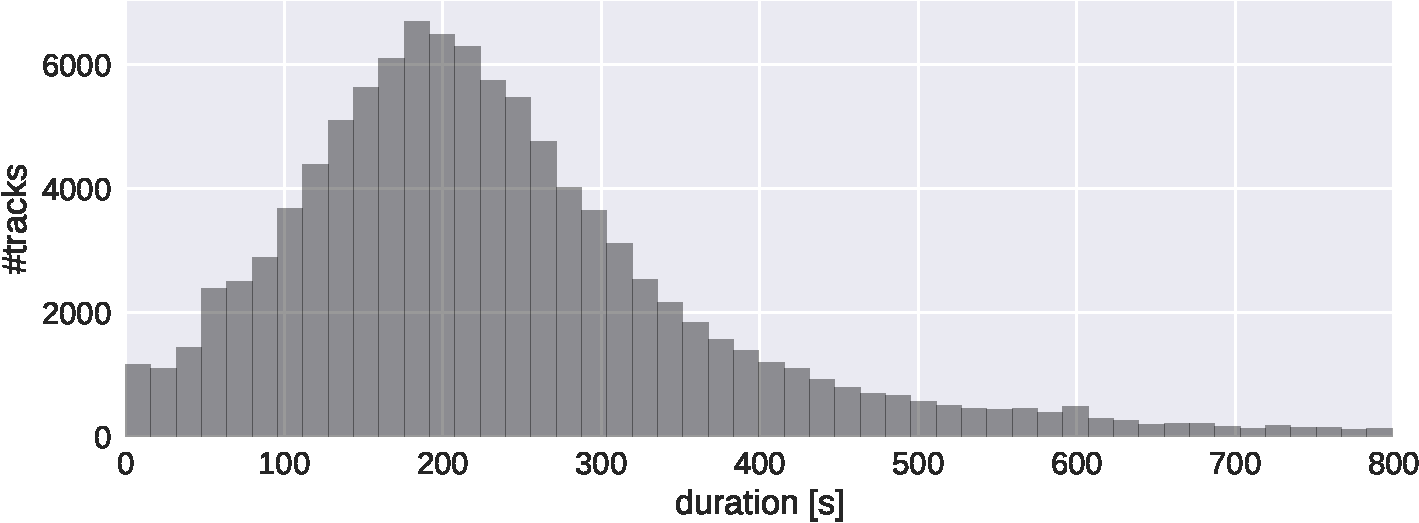
\includegraphics[width=\linewidth]{duration_distribution.pdf}
	\caption{Track duration, from 0 to 3 hours.}
	\label{fig:duration_distribution}
\end{figure}

\begin{figure}
	\centering
	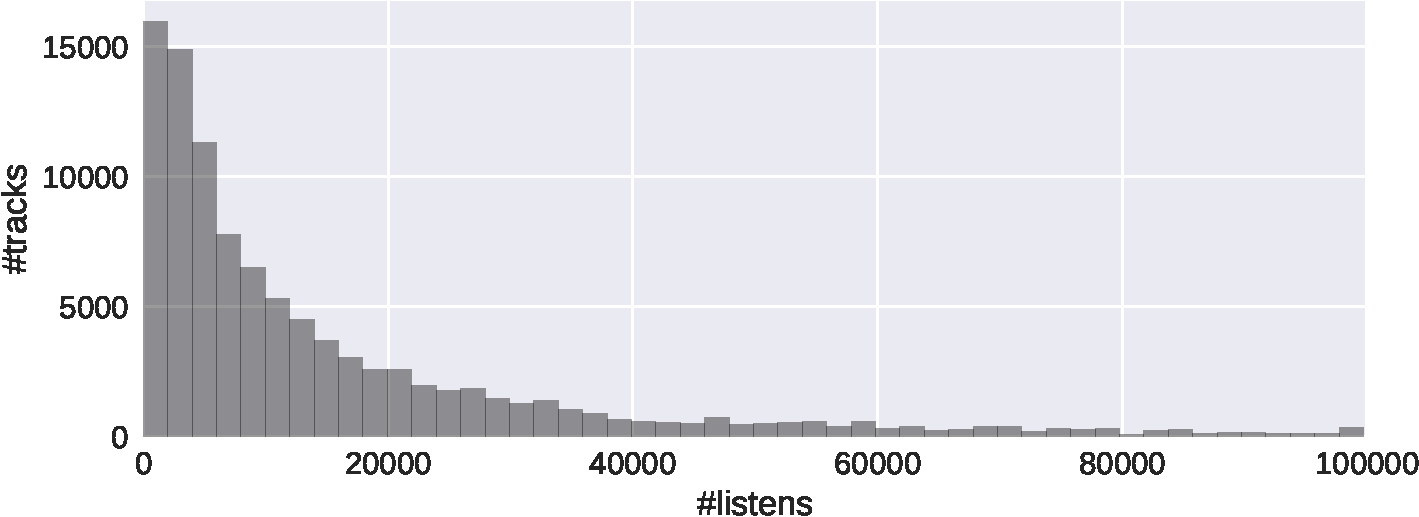
\includegraphics[width=\linewidth]{listens_distribution.pdf}
	\caption{Album listens, from 0 to 3.6 millions.}
	\label{fig:listens_distribution}
\end{figure}

\subsection{The Free Music Archive}

The dataset is a dump of the \href{https://freemusicarchive.org/}{Free Music Archive}, an interactive library of high-quality, legal audio downloads directed by \href{https://wfmu.org/}{WFMU}, the longest-running freeform radio station in the United States.
The archive is funded by the New York State Music Fund, the MacArthur Foundation, the National Endowment for the Arts, and from the project's users.
The website provides a large catalog of artists and high-quality mp3-encoded songs, hand-picked by established audio curators. Each song is legally free to download as artists decided to release their works under a permissive license, most tracks being released under a \href{https://creativecommons.org/}{Creative Commons license} which allows redistribution of the audio. Cheyenne Hohman, the director of the FMA, \href{http://freemusicarchive.org/member/cheyenne_h/blog/100000_SONGS}{announced} in July 2016 that the website had reached the landmark of 100,000 songs.
Inspired by Creative Commons and the open-source software movement, the FMA provides a legal and technological platform for curators, artists, and listeners to harness the potential of music sharing. While the archive is free and open to anyone, written and audio content is curated, and permission to upload or edit content is granted on an invitation basis \cite{art:MossFMA}.

\subsection{Creation} % Collection, Creation, Generation
% How it was collected.

% Collection
As of April 1st 2017, the date of collection, the online archive largest track id was 155,320, of which 109,727 were valid (the missing 45,594 ids probably correspond to deleted tracks). See \figref{fig:growth} to visualize the growth of the dataset. In addition to per-track metadata, the used hierarchy of 161 genres and extended album (480 not found) and artist (250 not found) information were collected via the available \href{https://freemusicarchive.org/api}{API}.\footnote{See \texttt{webapi.ipynb} to query the API with our helpers.}. Finally, mp3 audio was downloaded over HTTPS.
% Cleaning
Out of all collected track ids, 180 mp3s could not be downloaded, 286 could not be trimmed by ffmpeg, and features could not be extracted from 71. Finally, the license of 2,616 songs prohibited their redistribution, leaving us with \ntracks tracks.

%\subsection{Data Cleaning}
% classes with less than 1% of the number of tracks of the biggest class Pop/Rock are removed

%At this stage the number of genres is 138, but half have only a few samples. Thus we decided to only retain the genres with more than 100 samples. This defines a dataset of 77,643 music data with 68 genres. We further cleaned the dataset by removing tracks which belong to ``non-standard'' music genres like 'Noise', 'Garage', 'Sound Collage', 'Singer', 'Audio Collage', 'Glitch', 'Unclassifiable', 'Lo-Fi', 'Spoken', 'Poetry', 'Talk Radio', 'Avant-Garde', 'Experimental', 'Ambient', and 'Field Recording'. We also suppressed the songs with the title 'Untitled'. Besides, we decided to cut the long tail of the power law distribution by removing songs of genres with less than 300 songs.

\subsection{Content}
% Figures and tables from analysis.ipynb
% TODO audio properties: samplerate (% 44kHz), bitrate (% 128, VBR), channels (% mono, stereo)

The collected track, album and artist meta-informations\footnote{Raw data is available in \texttt{raw\_tracks.csv}, \texttt{raw\_albums.csv}, and \texttt{raw\_artists.csv}.} were cleaned, uniformly formatted, merged and stored in \texttt{tracks.csv}\footnote{See \texttt{creation.ipynb} for the code which created the dataset.} which \tabref{tab:tracks} shows an excerpt. That file is a relational table where each row represents a track and columns are listed in \tabref{tab:metadata}, although some values may be missing for some tracks. The audio for each track is stored in a file wich name is the track id. All songs are mp3-encoded, most of them with sampling rate of 44,100 Hz, bit rate 320 kb/s, and in stereo. Figures~\ref{fig:album_release_year},~\ref{fig:duration_distribution} and \ref{fig:listens_distribution} show the distribution of albums per year, track durations, and play counts per album.
See the \texttt{analysis.ipynb} notebook for a much more detailed analysis of the content.

%\todo{describe the metadata}

\subsection{Genres}

\begin{table}
	\centering
	\begin{tabular}{ccclr}
		\toprule
		id & parent & top\_level & title & \#tracks \\
		\midrule
		38 & None & 38 & Experimental & 38,154 \\
		15 & None & 15 & Electronic & 34,413 \\
		12 & None & 12 & Rock & 32,923 \\
		1235 & None & 1235 & Instrumental & 14,938 \\
		10 & None & 10 & Pop & 13,845 \\
		17 & None & 17 & Folk & 12,706 \\
		\midrule
		25 & 12 & 12 & Punk & 9,261 \\
		89 & 25 & 12 & Post-Punk & 1,858 \\
		1  & 38 & 38 & Avant-Garde & 8,693 \\
		\bottomrule
	\end{tabular}
	\caption{An excerpt of the genre hierarchy, stored in \texttt{genres.csv}. Some of the 16 top-level genres appear in the top part, while some second- and third-level genres appear in the bottom part.}
	\label{tab:genres}
\end{table}

While it is difficult to devise a hierarchy of genres, we followed that of our source. Indeed, the website offers a parent genre for each of the 163 available genres. \tabref{tab:genres} shows an excerp of that information along with the number of tracks per genre and the associated top-level genre, that is the root of the genre tree. \figref{fig:genre_hierarchy} shows an excerpt of the tree.
In the per-track table, the \texttt{genres} column contain the genre ids indicated by the artist. Then, given such hierarchical information, we constructed a \texttt{genres\_all} column which contains all the genres encountered when traversing the tree from the indicated genres to the roots. Finally, if the traversal yields only one root, the track is given a top-level genre stored in the \texttt{genre\_top} column.
\figref{fig:genre_distribution} shows the distribution of the most common genres. As often encountered with natural categories, it obeys a power law.
 
% MSD:
% not strictly genres (e.g. one of them is romantic dinner music)
% one non-music category

\begin{figure}
	\begin{minipage}[t]{0.44\linewidth}
		\centering
		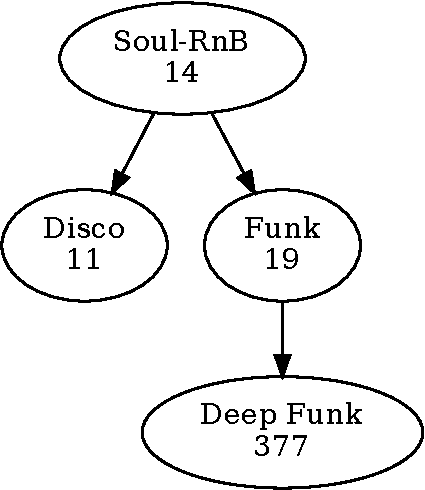
\includegraphics[width=\linewidth]{genre_hierarchy.pdf}
	\end{minipage} \hfill
	\begin{minipage}[t]{0.55\linewidth}
		\centering
		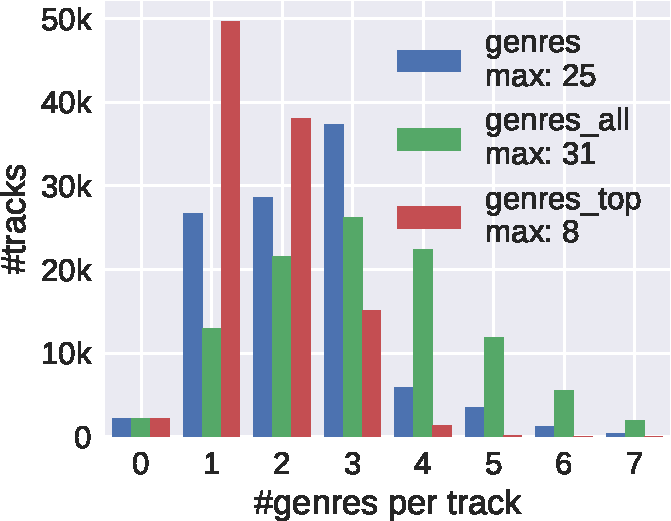
\includegraphics[width=\linewidth]{genres_per_track.pdf}
	\end{minipage}
	\caption{(left) Example of genre hierarchy for the top-level Soul-RnB genre. Left number is the \texttt{genre\_id}, right number is the number of tracks per genre. (right) Number of genres per track, from 0 to 31 (\texttt{genres\_all}).}
	\label{fig:genre_hierarchy}
	\label{fig:genres_per_track}
\end{figure}

\begin{figure}[t]
	\centering
	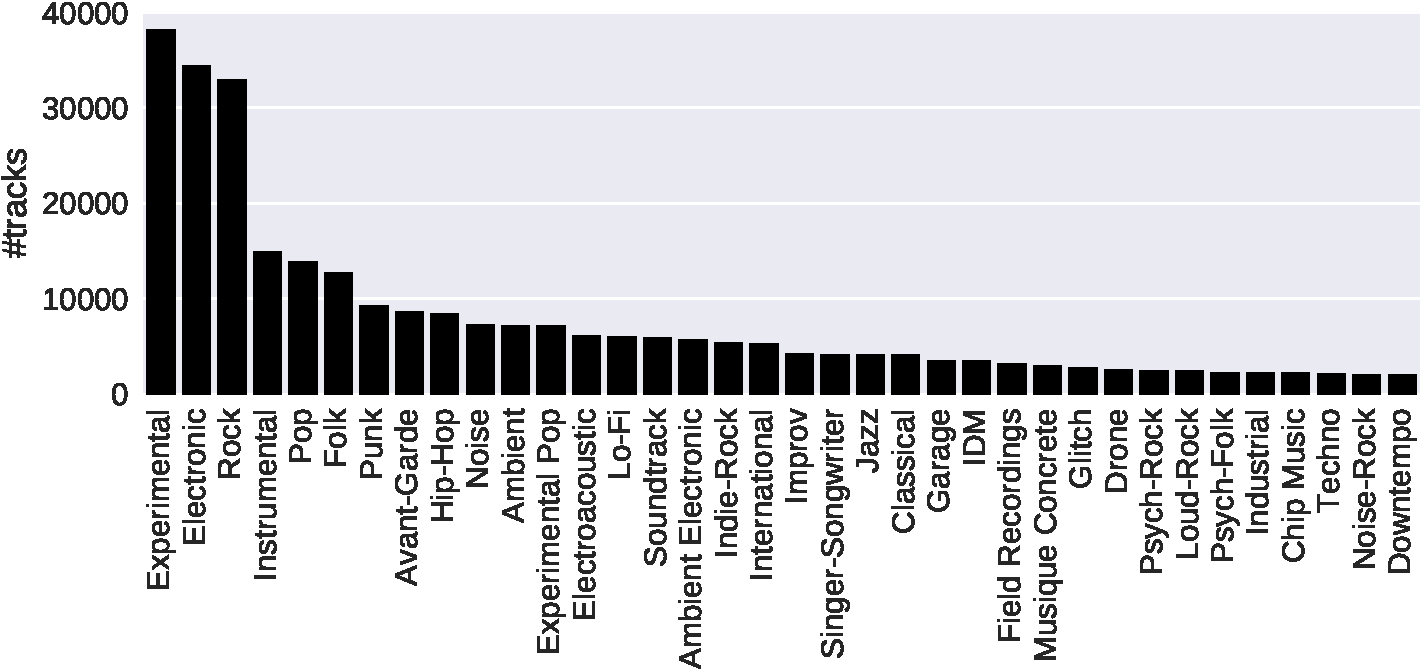
\includegraphics[width=\linewidth]{genre_distribution.pdf}
	\caption{Tracks per genre, from 1 to 38,154.}
	\label{fig:genre_distribution}
\end{figure}

\subsection{Features} % Feature sets

The upper part of \tabref{tab:features} lists the (mostly spectral) features we extracted from the audio with the \href{https://github.com/librosa/librosa}{librosa} Python library, version 0.5.0.
Each feature set (except zero-crossing rate) is computed on windows of 2048 samples spaced by hops of 512 samples. Seven statistics were then computed over all windows: the mean, standard deviation, skew, kurtosis, median, minimum and maximum.
Those 518 pre-computed features are distributed in \texttt{features.csv} for all tracks.\footnote{See \texttt{features.py} for the code which computed the features.}

In addition,
% a number of descriptive medium-level and high-level audio
features extracted by \href{http://the.echonest.com/}{Echonest}, a music platform, are provided for some tracks. These features include high-level audio features (acousticness, danceability, energy, instrumentalness, liveness, speechiness, tempo, valence), social features (artist discovery, artist familiarity, artist hotttness, song currency, song hotttness), and MFCC-like temporal features for a number of segments \cite{echonest_temporal}. They are distributed in \texttt{echonest.csv}.
%Echonest audio features are described in Kirell's paper
%Those features can be obtained either by uploading the songs to their website, which are then analyzed and sent back to the user, or simply retrieved from their database if the songs are known to them, i.e. they were analyzed before. All of which can be done through an \href{http://developer.echonest.com}{API}. In our case, we only retrieved features from songs which were already in their database.

\subsection{Subsets} \label{sec:subsets}

Finally, for the dataset to be useful as a development set or for people with lower computational resources, we propose the following subsets, each of which is a subset or the larger set:
\begin{enumerate}
	\item \textbf{Full}: the complete dataset, described above. All \ngenres genres, unbalanced with 1 to 38,154 tracks per genre (\figref{fig:genre_distribution}) and 0 to 31 genres per track (\figref{fig:genres_per_track}).
	\item \textbf{Large}: the full dataset with audio limited to 30 seconds clips extracted from the middle of the tracks (or entire song if shorter than 30 seconds). That trimming reduces the size of the data by a factor 10.
	\item \textbf{Medium}: 25,000 of the most popular tracks with good metadata and quality audio. Genre unbalanced with 21 to 7,103 tracks per top genre, but only one top genre per track.
	\item \textbf{Small}: 8,000 tracks from 8 top genres, balanced with 1000 tracks per genre, 1 genre per track. This subset is similar to the very popular GTZAN \cite{gtzan} with the added benefits of the FMA, that is metadata, pre-computed features, and copyright-free audio.
\end{enumerate}
\tabref{tab:subsets} highlights the main differentiating factors between the proposed subsets.
%See \texttt{analysis.ipynb} for an analysis of the subsets' content similar to that shown in \secref{sec:content}.

\subsection{Splits}

% PTB 19/3/3, MNIST 60/10, ImageNet 1200/50/100 --> ratio ~6-12
An 80/10/10\% split into training, validation and test sets is proposed to make research on the FMA reproducible. The training and validation sets should be merged if cross-validation is used instead.
Below are the constraints we followed:
% Data was stratified according to the following criteria: ground truth, artist and times filters
\begin{enumerate}
	\item Stratified sampling was used to preserve the percentage of tracks per genre. This is important for minority genres.
	\item An artist filter was used, i.e. an artist was forced to appear in one set only. %All songs from a given artist either appear in train, validation or test, never in two of them.
	%\item Stratified sampling with a time filter, i.e. for each genre using the earlier songs in the training set, and the later releases in the validation and test sets.
	\item Artists with lots of songs were distributed between the sets. %The three sets were alternatively filled in descending order of the count of artist songs. 
\end{enumerate}
The above constraints are satisfied for all subsets, and a track is assigned to the same split across all of them. See \texttt{creation.ipynb} for full details.

\begin{table}
	\centering
	\begin{tabular}{lrrccc}
		\toprule
		dataset & clips & genres & length & \multicolumn{2}{c}{size} \\
		\cmidrule{5-6}
		        &       &        &  [s]   & [GB] & [days] \\
		\midrule
		small  &    8,000 &   8 &  30 & 3.4  & 2.8  \\
		medium &   25,000 &  16 &  30 & 12.2 & 8.7  \\
		large  & \ntracks & 161 &  30 & 90   & 37 \\
		full   & \ntracks & 161 & \aduration & \size & \tduration  \\
		\bottomrule
	\end{tabular}
	\caption{Proposed subsets of the FMA.}
	\label{tab:subsets}
\end{table}


%%%%%%%%%%%%%%%%%%%%%%%%%%%%%%%%%%%%%%%%%%%%%%%%%%%%%%%%%%%%%%%%%%%%%%%%%%%%%%%%
\section{Proposed usage} % tasks, usage, problems
%%%%%%%%%%%%%%%%%%%%%%%%%%%%%%%%%%%%%%%%%%%%%%%%%%%%%%%%%%%%%%%%%%%%%%%%%%%%%%%%
% List some MIR tasks and propose some who can be done with that dataset


With its rich set of metadata, user data, audio and features, the FMA is amenable to many tasks in MIR. We share below some possible uses, which serves to illustrate the breadth of data available in the dataset.

% Metadata analysis
% Recommendation / Recommender systems, Music Similarity
% Music classification
	% Genre recognition / classification
	% Artist identification / recognition
	% Year prediction / recognition
% Automatic (music) tagging / autotagging --> tag prediction

%On an other hand, unsupervised learning methods could be used for music categorization. Does genre emerge? How?

% Segmentation
% Visualization
% Musicology

%\subsection{Album covers}
% image covers: generate covers per genre / artist
% study the influence of covers on ratings

\subsection{Metadata Analysis}

While the original intention of the dataset was to release a large volume of audio for machine learning algorithms, analyzing metadata from such a collection is also extremely interesting.
For instance, one could address questions like: How broads artists are, i.e. to which genres do they contribute to? Do we observe some drift in time for the vocabulary used in song titles, album names or artist names? To which extent tags correspond to genres? What other semantic categories can we found in them?
Other lines of work are to test algorithms for the imputation of missing data, or to study to what extent is the FMA representative of mainstream music, or how similar it is to other datasets.

\subsection{Recommendation} % Recommender Systems}
% Cite Kirell's paper: Song recommendation with non-negative matrix factorization and graph total variation

Due to the potential commercial value of a working system, music recommendation and music similarity are ones of the best studied areas of MIR. So far, content-based systems have fallen short at predicting user ratings when compared to collaborative filtering methods.
The availability of user data such as play counts for tracks and albums as well as number of comments and favorites for tracks, albums and artists opens the possibility of a large-scale evaluation of content-based recommender systems based on rich metadata, audio, or derived features, with a clean ground truth.

\subsection{Music Classification and Annotation}
%\subsection{Automatic Music Tagging}

\begin{figure}
	\centering
	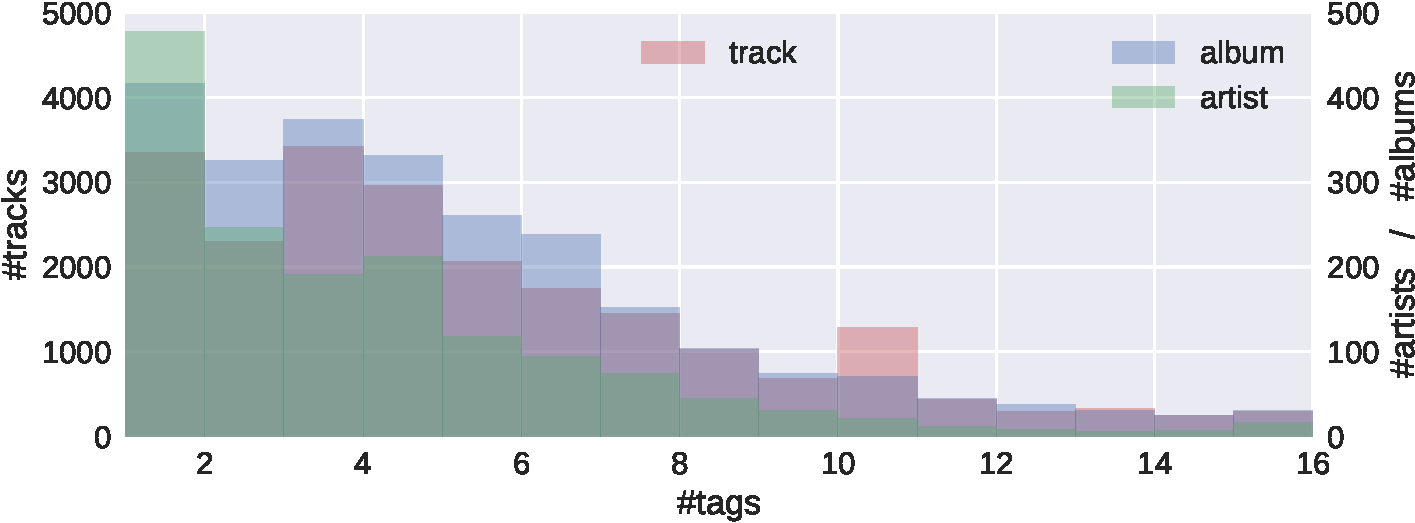
\includegraphics[width=\linewidth]{tag_distribution.pdf}
	\caption{Per-track, album and artist tags, from 0 to 150.}
	\label{fig:tag_distribution}
\end{figure}

Music classification is a key problem in MIR with many potential applications. For one, a classification system enables end users to search for the types of music they are interested in. On the other hand, different music types are managed more effectively and efficiently once they are categorized into different groups \cite{mir_review_classif}.
The classification tasks which can be evaluated on the available labels for the FMA include genre recognition, artist identification, year prediction, and music annotation. Automatic tagging is a classification problem which cover different semantic categories, where tags are labels which can be any musical term that describes the genre, mood, instrumentation, and style of the song.
%The task of music annotation has recently gained much popularity in the MIR community.
In the FMA, tags can be found at the track, album and artist level: 23,496 tracks (22\%), 2,659 albums (18\%) and 1,605 artists (10\%) have at least one tag. \figref{fig:tag_distribution} shows their distribution.\footnote{One of the artist tag is often the artist name, which we subtracted in our counts.}

\subsection{Limitations}
% ground truth for genre: AllMusic Guide (album, artist), Gracenote CDDB (song)
% musicbrainz, playme, 7digital
% Allmusic: album reviews, artist biographies, discographies as well as classification of albums according to genres, styles, moods and themes. Information is provided and curated by experts.

% Cover song recognition
% Lyrics
% Automatic playlist generation
% style?
% Music classification
	% mood classification,
	% instrument recognition / identification
	% music annotation --> temporal labels, e.g. instrument / note

% metadata such as genre, mood, groove, composer, performer, lyrics, meter, chord progressions, instruments present

While the FMA can be used to evaluate many tasks, metadata is missing for e.g. cover song recognition, mood classification or instrument recognition.
We can however expect people to cross-reference the dataset with other resources to unlock additional tasks, as has happened for example with the MSD and \href{http://www.allmusic.com}{AllMusic}, \href{https://www.last.fm}{last.fm} and \href{https://beatunes.com}{beaTunes} for genre recognition \cite{msd_features, msd_genres}, \href{https://musixmatch.com}{musixmatch} for lyrics, \href{https://secondhandsongs.com}{SecondHandSongs} for cover songs, or \href{https://www.thisismyjam.com}{This Is My Jam} for user play counts.

Diversity is another issue: as suggested by \figref{fig:genre_distribution}, this collection is biased toward experimental music, electronic and rock. Moreover, it probably does not contain hits from renown artists or commercial music.


%%%%%%%%%%%%%%%%%%%%%%%%%%%%%%%%%%%%%%%%%%%%%%%%%%%%%%%%%%%%%%%%%%%%%%%%%%%%%%%%
\section{Genre Recognition} % MGR, Baselines
%%%%%%%%%%%%%%%%%%%%%%%%%%%%%%%%%%%%%%%%%%%%%%%%%%%%%%%%%%%%%%%%%%%%%%%%%%%%%%%%


Music genres are categories that have arisen through a complex interplay of cultures, artists, and market forces to characterize similarities between compositions and organize music collections. Yet, the boundaries between genres still remain fuzzy, making the problem of music genre recognition (MGR) a nontrivial task.
% genre not defined by audio content only
While its utility has been debated, mostly because of its ambiguity and cultural definition, it is widely used and understood by end-users who find it useful to discuss musical categories \cite{mgr_why}.
As such, it is one of the most researched areas of MIR.
%\subsection{Data}
The FMA is especially suited for MGR as it features fine genre information, i.e. multiple genres associated to individual songs, has a built-in genre hierarchy (\tabref{tab:genres}), and is annotated by the artists themselves.
% While there certainly is noise in our labels, we trust the artists to have selected the most appropriate set of genres for their own songs.
Genre recognition problems of increasing difficulty are:
\begin{enumerate}
	\item Single top genre prediction on the small subset.
	\item Single top genre prediction on the medium subset.
	\item Multiple top genres prediction on the large / full set.
	\item Multiple genres prediction on the large / full set.
\end{enumerate}

%\subsection{Methods}
%\subsection{Evaluation and results}

\tabref{tab:mgr} reports classification accuracies for problem 2 with 9 different mainstream feature sets and some combinations as well as 4 standard classifiers using scikit-learn \cite{scikit-learn}, version 0.18.1. Specifically, we employed linear regression (LR) with an $L^2$ penalty, k-nearest neighbors (kNN) with $k=200$, support vector machines (SVM) with a radial basis function (RBF) kernel and a multilayer perceptron (MLP) with 100 hidden neurons. All classifiers were tested with mostly default settings.\footnote{See \texttt{baselines.ipynb} for all details.} Reported performances should not be taken as the state-art-of-the-art but rather as a lower-bound and an indication of the task's difficulty. Moreover, the produced code can serve as a reference and is easily modified to accommodate other features and classifiers.

% As a preliminary result, we trained a convolutional neural network on 3sec-spectrograms, and we select the class by majority voting.

While MGR has been MIR's flagship application for a while, prediction accuracy reached a glass ceiling \cite{mgr_why}.
A major motivation to construct this dataset was to enable the use of the powerful deep learning set of techniques to music analysis.
%thanks to the advent of specialized DL architectures with testable performances which can be compared.
With availability of audio, DL architectures such as convolutional neural networks and recurrent neural networks can be applied to the waveform to avoid any feature engineering. While those approaches have fallen behind learning from higher-level representations such as spectrograms \cite{dieleman_endtoend}, a greater exploration of the design space will hopefully provide alternatives to solving MIR challenges \cite{mir_dl_feature_learning}.

%Some very recent advances are indeed promising Chuo

\begin{table}
	\centering
	\begin{tabular}{l@{\tspaceb}r@{\tspaceb}c@{\tspaceb}c@{\tspaceb}c@{\tspaceb}c}
		\toprule
		feature set & dim. & LR & kNN & SVM & MLP \\
		\midrule
		1 Chroma \cite{chroma} & 84 & 44 & 44 & 48 & 49 \\
		2 Tonnetz \cite{tonnetz} & 42 & 40 & 37 & 42 & 41 \\
		3 MFCC \cite{mfcc} & 140 & 58 & 55 & 61 & 53 \\
		4 Spec. centroid & 7 & 42 & 45 & 46 & 48 \\
		5 Spec. bandwidth & 7 & 41 & 45 & 44 & 45\\
		6 Spec. contrast \cite{contrast} & 49 & 51 & 50 & 54 & 53 \\
		7 Spec. rolloff & 7 & 42 & 46 & 48 & 48 \\
		8 RMSE & 7 & 37 & 39 & 39 & 39 \\ % Root-mean-square energy
		9 Zero-crossing rate & 7 & 42 & 45 & 45 & 46 \\
		\midrule
		Ech. audio & 8 & - & - & - & - \\
		Ech. social & 5 & - & - & - & - \\
		Ech. temporal \cite{echonest_temporal} & 224 & - & - & - & - \\
		\midrule
		% Number and use them for aggregates
		3 + 6 & 189 & 60 & 55 & 63 & 54 \\
		3 + 6 + 4 & 273 & 60 & 55 & 63 & 53 \\
		1 to 9 & 518 & 61 & 52 & 63 & 58 \\
		\bottomrule
	\end{tabular}
	\caption{Accuracies of various features and classifiers for top genre recognition on the medium subset.}
	\label{tab:mgr}
	\label{tab:features}
\end{table}


%%%%%%%%%%%%%%%%%%%%%%%%%%%%%%%%%%%%%%%%%%%%%%%%%%%%%%%%%%%%%%%%%%%%%%%%%%%%%%%%
\section{Conclusion and Perspectives}
%%%%%%%%%%%%%%%%%%%%%%%%%%%%%%%%%%%%%%%%%%%%%%%%%%%%%%%%%%%%%%%%%%%%%%%%%%%%%%%%
% MSD: the future of the dataset, visibility for MIR (to DL people!)

% importance of open data

Benchmarking is an important aspect in experimental sciences -- results reported by individual research groups need to be comparable. Important aspects of these are datasets that can be easily shared among researchers, together with a set of defined tasks and splits. The FMA enables researchers to test algorithms on a large-scale collection, closer to real-world environments. Even though it is still two orders of magnitude behind commercial services who have access to tens of millions of songs,\footnote{\href{http://the.echonest.com}{37M Echonest}, \href{https://en.wikipedia.org/wiki/Spotify}{30M Spotify}, \href{http://www.skilledtests.com/wiki/Last.fm_statistics}{45M last.fm}, \href{http://bupz.com/best-websites-to-buy-musics}{45M 7digital}, \href{https://www.apple.com/pr/library/2013/02/06iTunes-Store-Sets-New-Record-with-25-Billion-Songs-Sold.html}{26M iTunes}} it is of the same scale as the largest image dataset (see \tabref{tab:size}) which opened the door to dramatic performance improvements for many tasks in computer vision.
%is also far behind the amount of tagged photos \href{https://www.facebook.com}{Facebook} has access to for example.
By providing audio, we do not limit the benchmarking to pre-computed features and allow scientists to develop and test new feature sets, learn features, or learn mappings directly from the audio.
% talk about metadata ?
% Kirell: less DL oriented, some people don't like it. Insist on available audio.

% Once that problem is well advanced, researchers will be able to tackle more difficult tasks such as tagging or annotation.
% Besides, standard data analysis tasks such as classification, clustering, regression, text analysis, visualization can also be applied to this new music dataset.

% Future work
In addition to the proposed usage and many others people will find, future work on the dataset itself may consider to scrap the website for information not available through the API, e.g. the number of downloads or the user comments. Moreover, cross-referencing with other resources or crowd-sourcing (with e.g. \href{https://www.mturk.com}{Mechanical Turk} or \href{https://www.crowdflower.com/}{CrowdFlower}) is desirable to obtain additional labels or measure agreement on the current ones by independent annotators.

In a \href{https://freemusicarchive.org/member/cheyenne_h/blog/FMA_Dataset_for_Researchers}{blog post about this dataset}, Cheyenne Hohman, the Director at the Archive, wrote that "by embracing the some rights reserved philosophy of Creative Commons, artists are not only making their music available for the public to listen to, but also for educational and research applications".
% Let's hope the research community may contribute back and that we can engage in a mutually benefit.
% Maybe in some future utopia, those kind of collaborations could shape a future where sharing is first and researchers feed open platforms with their algorithms while they feed us with data. That would especially be useful for recommendation systems.

% Foster usage of CC and interplay between artists, platforms, users and researchers.


%%%%%%%%%%%%%%%%%%%%%%%%%%%%%%%%%%%%%%%%%%%%%%%%%%%%%%%%%%%%%%%%%%%%%%%%%%%%%%%%
\section{Acknowledgments}
%%%%%%%%%%%%%%%%%%%%%%%%%%%%%%%%%%%%%%%%%%%%%%%%%%%%%%%%%%%%%%%%%%%%%%%%%%%%%%%%


We want to thank the team supporting the \href{https://freemusicarchive.org}{Free Music Archive} as well as all the contributing artists and curators for the fantastic content they made available.
We are grateful to SWITCH and EPFL for hosting the dataset within the context of the \href{https://projects.switch.ch/scale-up}{SCALE-UP} project, funded in part by the swissuniversities \href{http://www.swissuniversities.ch/isci}{SUC P-2 program}.
% We are grateful to \href{https://zenodo.org}{zenodo.org}, whose free hosting and archiving of digital research artifacts is promoting a more open scientific process.
Xavier Bresson is supported by NRF Fellowship NRFF2017-10.

\bibliography{refs}
\end{document}
